\begin{flushright} {\tiny {\color{gray} mms\_generic3D.tex}} \end{flushright}
%~~~~~~~~~~~~~~~~~~~~~~~~~~~~~~~~~~~~~~~~~~~~~~~~~~~~~~~~~~~~~~~~~~~~~~~~~~~~~~~~~~~~~~~~~~~~~~~~~~

We postulate
\begin{eqnarray}
u(x,y,z) &=& f(x) g'(y) h'(z) \\
v(x,y,z) &=& f'(x) g(y) h'(z) \\
w(x,y,z) &=& -2f'(x) g'(y) h(z) 
\end{eqnarray}
so that the flow is indeed incompressible: 
\[
\frac{\partial u}{\partial x}+
\frac{\partial v}{\partial y}+
\frac{\partial w}{\partial z}
=
f'(x) g'(y) h'(z) + f'(x) g'(y) h'(z) -2f'(x) g'(y) h'(z)
=0
\]
The velocity gradient ${\bm L}(\vec\upnu)$ is then given by
\[
{\bm L}(\vec\upnu) =
\left(
\begin{array}{ccc}
f'g'h' &  f'' g h' & -2f'' g' h \\ \\
fg''h' & f'g'h'    & -2f' g'' h \\ \\
fg'h'' & f'gh''    & -2f'g'h'
\end{array}
\right)
\]
and the strain rate tensor by:
\[
\dot{\bm \varepsilon}(\vec\upnu)
=\frac{1}{2}({\bm L}(\vec\upnu)+{\bm L}(\vec\upnu)^T)
=
\frac{1}{2}
\left(
\begin{array}{ccc}
2f'g'h' & (f'' g+fg'') h'  & fg'h''-2f'' g' h \\ \\
(f''g+fg'')h' & 2f'g'h'    & f'gh''-2f' g'' h \\ \\
fg'h'' -2f'' g' h & f'gh'' -2f' g'' h    & -4f'g'h'
\end{array}
\right)
\]

We assume for simplicity that $\eta=1$ so 
\begin{eqnarray}
\vec\nabla\cdot 2\eta \dot{\bm \varepsilon}(\vec\upnu)
&=&
\vec\nabla\cdot \left(
\begin{array}{ccc}
2f'g'h'           & (f'' g+fg'') h'    & fg'h''-2f'' g' h \\ \\
(f''g+fg'')h'     & 2f'g'h'            & f'gh''-2f' g'' h \\ \\
fg'h'' -2f'' g' h & f'gh'' -2f' g'' h  & -4f'g'h'
\end{array}
\right) \nn\\
&=&
\left(
\begin{array}{c}
2f''g'h' +    (f''g'+fg''')h'   +   fg'h''' -2f'' g' h'   \\ \\
(f''' g+f'g'') h'  +     2f'g''h'   +     f'gh''' -2f' g'' h' \\ \\
f'g'h''-2f''' g' h   +  f'g'h''-2f' g''' h     -4f'g'h''
\end{array}
\right) \nn\\
&=&
\left(
\begin{array}{c}
f''g' h'  + fg''' h'  +  fg'h'''   \\ \\
f''' g h' + f'g'' h'  +  f'gh'''  \\ \\
-2f''' g' h     -2f' g''' h -2f'g'h''
\end{array}
\right) 
\end{eqnarray}
The Stokes equation then writes 
\[
\left(
\begin{array}{c}
-\partial_x p \\ \\
-\partial_y p \\ \\
-\partial_z p 
\end{array}
\right) 
+
\left(
\begin{array}{c}
f''g' h'  + fg''' h'  +  fg'h'''   \\ \\
f''' g h' + f'g'' h'  +  f'gh'''  \\ \\
-2f''' g' h     -2f' g''' h -2f'g'h''
\end{array}
\right) 
+
\left(
\begin{array}{c}
b_x \\ \\ b_y \\ \\ b_z
\end{array}
\right) 
=\vec{0}
\]
or, 
\[
\left(
\begin{array}{c}
b_x \\ \\ b_y \\ \\ b_z
\end{array}
\right) 
=
\left(
\begin{array}{c}
\partial_x p \\ \\
\partial_y p \\ \\
\partial_z p 
\end{array}
\right) 
-
\left(
\begin{array}{c}
f''g' h'  + fg''' h'  +  fg'h'''   \\ \\
f''' g h' + f'g'' h'  +  f'gh'''  \\ \\
-2f''' g' h     -2f' g''' h -2f'g'h''
\end{array}
\right) 
\]

%..............................
\paragraph{First application}


Let us assume 
\[
f(x)=x(1-x) \qquad
g(y)=y(1-y) \qquad
h(z)=z(1-z) 
\]
then 
\[
f'(x)=1-2x \qquad
g'(y)=1-2y \qquad
h'(z)=1-2z 
\]
\[
f''(x)=-2 \qquad
g''(y)=-2 \qquad
h''(z)=-2 
\]
\[
f'''(x)=0 \qquad
g'''(y)=0 \qquad
h'''(z)=0 
\]
Which ensures that there is no flow through the boundaries of the unit cube.
Then 
\[
\left(
\begin{array}{c}
b_x \\ \\ b_y \\ \\ b_z
\end{array}
\right) 
=
\left(
\begin{array}{c}
\partial_x p \\ \\
\partial_y p \\ \\
\partial_z p 
\end{array}
\right) 
-
\left(
\begin{array}{c}
f''g' h'     \\ \\
f'g'' h'    \\ \\
-2f'g'h''
\end{array}
\right) 
\]
with 
\begin{eqnarray}
u(x,y,z) &=& x(1-x)(1-2y)(1-2z)\\
v(x,y,z) &=& (1-2x) y(1-y) (1-2z) \\
w(x,y,z) &=& -2(1-2x)(1-2y)z(1-z)
\end{eqnarray}

Finally we postulate 
\[
p(x,y,z) = (2x-1)(2y-1)(2z-1)
\]
with $\int_\Omega p(x,y,z) dx dy dz =0$, so
\[ 
\left(
\begin{array}{c}
\partial_x p \\ \\
\partial_y p \\ \\
\partial_z p 
\end{array}
\right) 
=
\left(
\begin{array}{c}
2(2y-1)(2z-1) \\\\
2(2x-1)(2z-1) \\\\
2(2x-1)(2y-1) 
\end{array}
\right) 
\]
Then we find that 
\[
\vec{b}
=
\left(
\begin{array}{c}
2(2y-1)(2z-1) -(-2)(1-2y)(1-2z) \\
2(2x-1)(2z-1) -(1-2x)(-2)(1-2z) \\
2(2x-1)(2y-1) +2(1-2x)(1-2y)(-2)
\end{array}
\right)
=
\left(
\begin{array}{c}
4(2y-1)(2z-1)\\ \\
4(2x-1)(2z-1) \\ \\
-2(2x-1)(2y-1) 
\end{array}
\right)
\]


The root mean square velocity is given by 
\begin{eqnarray}
\int_\Omega u^2 dV &=& 1/270 \\
\int_\Omega v^2 dV &=& 1/270 \\
\int_\Omega w^2 dV &=& 2/135
\end{eqnarray}
and then 
\[
\upnu_{vrms} =\sqrt{\frac{6}{270}} \simeq 0.1490712
\]

This benchmark is implemented in \stone~\ref{f10} ($Q_1\times P_0$), 
\stone~\ref{f75} (MINI-1 bubble) 
and \stone~\ref{f82} (MINI-2 bubbles).  
The code is available in {\tt /mms/mms3D.py}.

\begin{center}
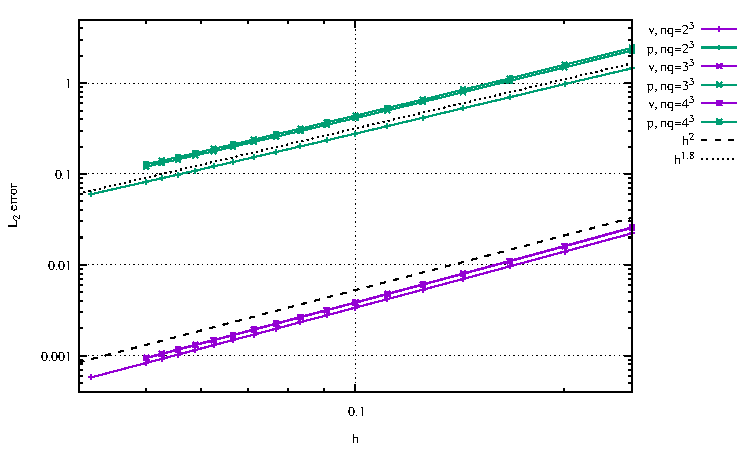
\includegraphics[width=8cm]{images/mms/generic3D/conv.pdf}
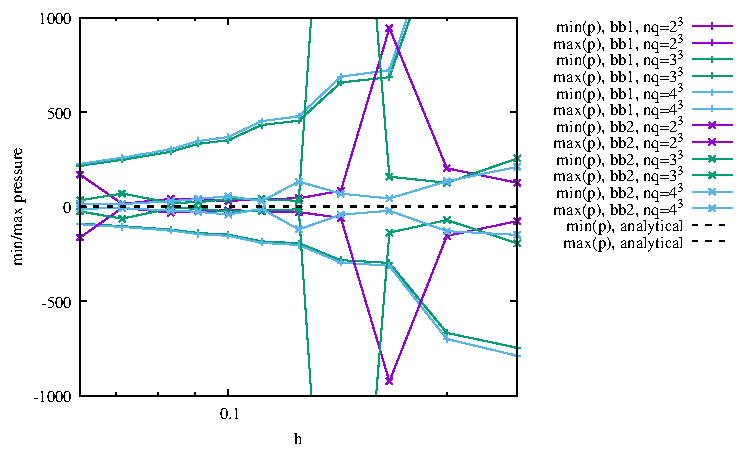
\includegraphics[width=8cm]{images/mms/generic3D/p_stats.pdf}\\
{\captionfont Error convergence and pressure statistics}
\end{center}

%..................................
\paragraph{Second application}

Once again, no flow through the boundaries of the unit cube:
\[
f(x)=x^2(1-x)^2 \qquad
g(y)=y^2(1-y)^2 \qquad
h(z)=z^2(1-z)^2 
\]
then 
\[
f'(x)=2x(2x^2-3x+1) \qquad
g'(y)=2y(2y^2-3y+1) \qquad
h'(z)=2z(2z^2-3z+1) 
\]
\[
f''(x)=2(6x^2-6x+1) \qquad
g''(y)=2(6y^2-6y+1) \qquad
h''(z)=2(6z^2-6z+1)
\]
\[
f'''(x)=24x-12 \qquad
g'''(y)=24y-12 \qquad
h'''(z)=24z-12
\]
The velocity field is then given by
\begin{eqnarray}
u(x,y,z) 
&=& f(x) g'(y) h'(z) 
= 4 x^2(1-x)^2  y(2y^2-3y+1) z(2z^2-3z+1)  \nn\\
v(x,y,z) 
&=& f'(x) g(y) h'(z) 
= 4 x(2x^2-3x+1) y^2(1-y)^2 z(2z^2-3z+1) \nn\\
w(x,y,z) 
&=& -2f'(x) g'(y) h(z) 
= -8 x(2x^2-3x+1) y(2y^2-3y+1) z^2(1-z)^2 
\end{eqnarray}
We choose
\[
p(x,y,z)=f'g'h' = 2x(2x^2-3x+1)  2y(2y^2-3y+1)  2z(2z^2-3z+1) 
\]
















